\clearpage
\VerdierPhysicalPageAnchor{0099}%
\begingroup
\setlength{\abovedisplayskip}{3pt plus 2pt minus 2pt}%
\setlength{\belowdisplayskip}{3pt plus 2pt minus 2pt}%
\setlength{\jot}{2pt}%
\VerdierSemanticAnchor{ch1-3-3-5-condition-a}
\noindent\textit{a) 令图}

\VerdierSemanticAnchor{ch1-3-3-5-morphism-triangles-first}
\begin{center}
  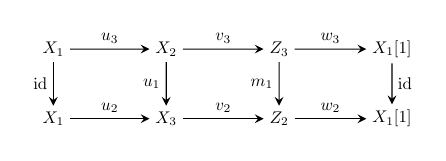
\begin{tikzpicture}[>=stealth,scale=0.61,every node/.style={transform shape}]
    \node (X1t) at (0,1.45) {$X_1$};
    \node (X2t) at (2.35,1.45) {$X_2$};
    \node (Z3t) at (4.70,1.45) {$Z_3$};
    \node (X1st) at (7.05,1.45) {$X_1[1]$};
    \node (X1b) at (0,0) {$X_1$};
    \node (X3b) at (2.35,0) {$X_3$};
    \node (Z2b) at (4.70,0) {$Z_2$};
    \node (X1sb) at (7.05,0) {$X_1[1]$};
    \draw[->] (X1t) -- node[above] {$u_3$} (X2t);
    \draw[->] (X2t) -- node[above] {$v_3$} (Z3t);
    \draw[->] (Z3t) -- node[above] {$w_3$} (X1st);
    \draw[->] (X1b) -- node[above] {$u_2$} (X3b);
    \draw[->] (X3b) -- node[above] {$v_2$} (Z2b);
    \draw[->] (Z2b) -- node[above] {$w_2$} (X1sb);
    \draw[->] (X1t) -- node[left] {$\mathrm{id}$} (X1b);
    \draw[->] (X2t) -- node[left] {$u_1$} (X3b);
    \draw[->] (Z3t) -- node[left] {$m_1$} (Z2b);
    \draw[->] (X1st) -- node[right] {$\mathrm{id}$} (X1sb);
  \end{tikzpicture}
\end{center}
\VerdierSemanticAnchor{ch1-3-3-5-morphism-triangles-second}
\begin{center}
  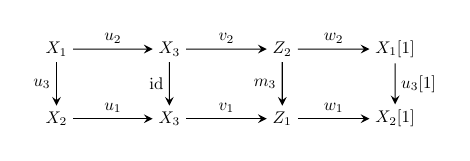
\begin{tikzpicture}[>=stealth,scale=0.61,every node/.style={transform shape}]
    \node (X1t) at (0,1.45) {$X_1$};
    \node (X3t) at (2.35,1.45) {$X_3$};
    \node (Z2t) at (4.70,1.45) {$Z_2$};
    \node (X1st) at (7.05,1.45) {$X_1[1]$};
    \node (X2b) at (0,0) {$X_2$};
    \node (X3b) at (2.35,0) {$X_3$};
    \node (Z1b) at (4.70,0) {$Z_1$};
    \node (X2sb) at (7.05,0) {$X_2[1]$};
    \draw[->] (X1t) -- node[above] {$u_2$} (X3t);
    \draw[->] (X3t) -- node[above] {$v_2$} (Z2t);
    \draw[->] (Z2t) -- node[above] {$w_2$} (X1st);
    \draw[->] (X2b) -- node[above] {$u_1$} (X3b);
    \draw[->] (X3b) -- node[above] {$v_1$} (Z1b);
    \draw[->] (Z1b) -- node[above] {$w_1$} (X2sb);
    \draw[->] (X1t) -- node[left] {$u_3$} (X2b);
    \draw[->] (X3t) -- node[left] {$\mathrm{id}$} (X3b);
    \draw[->] (Z2t) -- node[left] {$m_3$} (Z1b);
    \draw[->] (X1st) -- node[right] {$u_3[1]$} (X2sb);
  \end{tikzpicture}
\end{center}
\VerdierSemanticAnchor{ch1-3-3-5-condition-a-conclusion}
\textit{为三角的态射。}

\VerdierSemanticAnchor{ch1-3-3-5-condition-b}
\noindent\textit{b) 令三角}
\VerdierSemanticAnchor{ch1-3-3-5-z-triangle}
\[
  Z_3\xrightarrow{m_1}Z_2\xrightarrow{m_3}Z_1
  \xrightarrow{v_3[1]w_1}Z_3[1]
\]
\VerdierSemanticAnchor{ch1-3-3-5-condition-b-conclusion}
\textit{为特异三角。}

\VerdierSemanticAnchor{ch1-3-3-5-proof}
取 $\operatorname{comp}(C)$ 的态射
$f\colon X_1\longrightarrow X_2$（分别地，
$g\colon X_2\longrightarrow X_3$），使其属于类 $\dot u_3$
（分别地，$\dot u_1$）。
\VerdierSemanticAnchor{ch1-3-3-5-composite}
令 $h=gf\colon X_1\longrightarrow X_3$。态射 $h$ 属于类
$\dot u_2$。为证明该命题，只需取 (3.2.2) 中的三角为特异三角：

\VerdierSemanticAnchor{ch1-3-3-5-cone-triangles}
\begin{align*}
  X_1&\xrightarrow{\dot f}X_2\xrightarrow{\dot p(f)}c(f)
       \xrightarrow{\dot q(f)}X_1[1],\\
  X_2&\xrightarrow{\dot g}X_3\xrightarrow{\dot p(g)}c(g)
       \xrightarrow{\dot q(g)}X_2[1],\\
  X_1&\xrightarrow{\dot h}X_3\xrightarrow{\dot p(h)}c(h)
       \xrightarrow{\dot q(h)}X_1[1]
\end{align*}
\VerdierSemanticAnchor{ch1-3-3-5-cone-morphisms}
并取下列态射为相应的态射：
\[
  c(D)\colon c(f)\longrightarrow c(h),
  \qquad
  c(D')\colon c(h)\longrightarrow c(g),
\]
其中 $D$ 与 $D'$ 是图

\VerdierSemanticAnchor{ch1-3-3-5-d-squares}
\begin{center}
  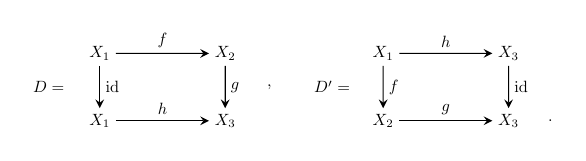
\begin{tikzpicture}[>=stealth,scale=0.59,every node/.style={transform shape}]
    \node at (-1.05,0.73) {$D={}$};
    \node (X1t) at (0,1.45) {$X_1$}; \node (X2t) at (2.70,1.45) {$X_2$};
    \node (X1b) at (0,0) {$X_1$};    \node (X3b) at (2.70,0) {$X_3$};
    \draw[->] (X1t) -- node[above] {$f$} (X2t);
    \draw[->] (X1t) -- node[right] {$\mathrm{id}$} (X1b);
    \draw[->] (X2t) -- node[right] {$g$} (X3b);
    \draw[->] (X1b) -- node[above] {$h$} (X3b);
    \node at (3.65,0.73) {$,$};
    \node at (5.05,0.73) {$D'={}$};
    \node (Y1t) at (6.10,1.45) {$X_1$}; \node (Y3t) at (8.80,1.45) {$X_3$};
    \node (Y2b) at (6.10,0) {$X_2$};    \node (Y3b) at (8.80,0) {$X_3$};
    \draw[->] (Y1t) -- node[above] {$h$} (Y3t);
    \draw[->] (Y1t) -- node[right] {$f$} (Y2b);
    \draw[->] (Y3t) -- node[right] {$\mathrm{id}$} (Y3b);
    \draw[->] (Y2b) -- node[above] {$g$} (Y3b);
    \node at (9.70,0.00) {$.$};
  \end{tikzpicture}
\end{center}
\endgroup

